%% Copernicus Publications Manuscript Preparation Template for LaTeX Submissions
%% ---------------------------------
%% This template should be used for the following class files: copernicus.cls, copernicus2.cls, copernicus_discussions.cls
%% The class files, the Copernicus LaTeX Manual with detailed explanations regarding the comments
%% and some style files are bundled in the Copernicus Latex Package which can be downloaded from the different journal webpages.
%% For further assistance please contact the Publication Production Office (production@copernicus.org).
%% http://publications.copernicus.org


%% Differing commands regarding the specific class files are highlighted.


%% copernicus.cls
\documentclass[gmd]{copernicus}
\usepackage{color}
%% copernicus2.cls
%\documentclass[journal abbreviation]{copernicus2}

%% copernicus_discussions.cls
%\documentclass[journal abbreviation, hvmath, online]{copernicus_discussions}


\begin{document}

\linenumbers

\title{NCAR Global Model Topography Generation Software for Unstructured Grids}


\author[1]{Julio T. Bacmeister}
\author[1]{Peter H. Lauritzen}
\author[1]{Patrick F. Callaghan}

\affil[1]{National Center for Atmospheric Research, 1850 Table Mesa Drive, Boulder, Colorado, USA}
%\affil[2]{ADDRESS}

%% The [] brackets identify the author to the corresponding affiliation, 1, 2, 3, etc. should be inserted.



\runningtitle{topo}

\runningauthor{Lauritzen et al.}

\correspondence{Peter Hjort Lauritzen\\ (pel@ucar.edu)}


\received{??}
%\pubdiscuss{} %% only important for two-stage journals
%\revised{}
%\accepted{}
%\published{}

%% These dates will be inserted by the Publication Production Office during the typesetting process.


\firstpage{1}

\maketitle  %% Please note that for the copernicus2.cls this command needs to be inserted after \abstract{TEXT}



\begin{abstract}
TEXT
\end{abstract}



\introduction  %% \introduction[modified heading if necessary]
Accurate representation of the impact of topography on atmospheric flow is crucial for Earth system modeling.  For example, on the regional scale the hydrological cycle is closely linked to topography and, on the planetary scale, waves associated with the mid-latitude jets are very susceptible to the effective drag caused by mountains \citep[e.g., ][]{LM1997QJRMS}. Atmospheric blocking producing heat waves and droughts as well as atmospheric rivers are closely related to topographic forcing. Despite the fact that surface elevation is known globally to within a meter (or less), its representation in numerical models remains a challenge.

The interaction between topography and dynamics in numerical models is usually split into to components:
\begin{itemize}
\item Resolved scale representation of topography in the dynamical core.
\item Representation of sub-grid processes: e.g. unresolved gravity waves, low-level jet blocking, and turbulence forced by topography that result in a mean drag on the resolved-scale flow.
\end{itemize}
These two components are discussed in sub-sections below as well as the topographic input data typically needed by numerical models.
\subsection{Resolved-scale topography: Surface geopotential $\Phi_s$}
The resolved scale component is basically the surface geopotential, $\Phi_s$, which is related to the mean elevation in each grid box. The `raw' elevation data is usually from a digital elevation model (DEM) such as the GTOPO30; a 30 arc second global dataset from the United States Geological Survey \citep[USGS; ][]{USGS} defined on an approximately 1km regular latitude-longitude grid. Several newer, more accurate, and locally higher resolution elevation datasets are available such as GLOBE \citep{GLOBE} and the NASA Shuttle Radar Topographic Mission (SRTM) DEM data \citep{SRTM}. The SRTM data, however, is only near-global (up to 60$^\circ$ North and South).
% Currently the CESM uses the GTOPO30 dataset. The `raw' elevation data of choice is used to compute surface geopotential $\Phi_s$ for the dynamical core and sub-grid scale variance for parameterizations of topographic effects such as gravity wave drag and turbulent mountain stress.

For models based on a terrain-following coordinate the specification of $\Phi_s$ determines the location of vertical levels in that the levels closer to the surface has gradients proportional to the surface elevation. Hence the terrain-following coordinates are not perpendicular to the direction of the stratification (the radial direction) so errors can arise when calculations are needed along stratified layers. For example, the pressure-gradient force (PGF) in terrain-following coordinates splits into two terms; one that is proportional to the geopotential gradient and one that is proportional to the pressure gradient. These terms are of similar magnitude but opposite sign. For a perfectly balanced flow these terms should exactly cancel. Failure to preserve this balance can produce large spurious vertical velocities. This problem, referred to as the PGF error/problem, has significant implications for global atmospheric modeling, with efforts to tackle this problem stretching back as far as the late 1970s \citep{ZIJ1977BzPdA, DTMZIJ1986MAP}.  As global models reach finer spatial scales, the pressure gradient problem leads to an increasingly polluted dynamical solution near steep topography since an increase in horizontal resolution, in general, steepen slopes. 

When performing a spectral analysis of the raw elevation data, it is clear that Earth's topography decreases quite slowly with increasing wave number \citet[see, e.g., ][]{B1993GRL}. Consequently, there will always be a non-negligible spectral component of topography present near the grid scale at current and any foreseeable model resolution. It is common practice not to force the highest wave numbers directly in the model to alleviate obvious spurious noise \citep[e.g.][]{NSM1994JC,LH1997MWR}. Hence the raw topographic data is filtered to remove the highest wave numbers. There seem to be no standardized procedure, for example a test case suite, to objectively select level of smoothing and filtering method. 

While it is necessary to smooth topography to remove spurious grid-scale noise, it introduces two problems. Filtering will typically raise ocean points near step topography to non-zero elevation. Perhaps the most striking example is the Andes mountain range that extends one or two grid cells into the Pacific after the filtering operation (see, e.g., Figure \ref{fig:oro-spectra} right). Ocean and land points are treated separately in weather/climate models so raised sea-points may potentially be problematic. Secondly, the filtering will generally reduce the height of local topographic maxima and given the importance of barrier heights in atmospheric dynamics, this could be a problem for the global angular momentum budget and could fundamentally change the flow. 

To capture the barrier effect (blocking) that is sub-grid scale with respect to the smoothed topography, one may use {\em{envelope topography}} that adjusts the surface height with sub-grid scale topographic variance \citep{WTS1983QJRMS}. Loosely speaking, the peak heights are raised. A similar approach, but implemented as variational filtering, is taken in \cite{RTS2006QJRMS}; this method also imposes additional constraints such as enforcing zero elevation over ocean masks.

As mentioned above it is not straight forward to determine how to smooth topography. One approach is to try different filtering methods in the full model and evaluate the results in weather forecasts or longer climate simulations \citep{NSM1994JC,B1995QJRMS,H1996JC}. While this approach is certainly valuable, clearly the size of the Gibbs oscillations in global spectral models is reduced by smoothing topography, it does not take into account the interaction between the resolved-scale flow (dynamical core) and parameterizations of sub-grid scale processes (e.g., gravity wave drag, turbulent mountain stress). This interaction can be difficult to predict and commonly the sub-grid scale parameterization have been tuned over a number of years with the `default' smoothed surface elevation. Hence, this methodology runs the risk of deeming one smoothing less accurate than another due to lack of optimum tuning (and/or complexity) of the parameterizations.

Another approach is to use idealized simulation with no parameterizations to determine what scales are adequately resolved and which are poorly resolved. \cite{DB2001QJRMS} kept the physical scale of an idealized two-dimensional and three-dimensional isolated hill fixed and observed how the coarser resolution results differ from the high-resolution simulation. This can then provide guide-lines on how to smooth topography in the full model. Similar idealized (shallow water) experiments where used in \cite{RTS2006QJRMS} to optimally smooth topography. While these idealized tests provide a `cleaner' approach to smoothing terrain, they do not consider the coupling with sub-grid scale processes.


\subsection{Sub-grid-scale topography: }
On the sub-grid scale there are many processes associated with topography such as sub-grid blocking, flow splitting, sheltering effects, generation of turbulence by roughness and gravity wave breaking \citep{B1990BAMS}. Only a brief overview of common parameterizations is given here.

Turbulent drag may be parameterized either through `effective roughness lengths' \citep{FP1972WJRMS} or  specified with an explicit topographic stress profile (introduced by \citet{WBH2001QJRMS} and used by \citet{BBW2004QJRMS}). These parameterizations are referred to as turbulent mountain stress (TMS); a form drag exerted by sub-grid scale topography \citep[][]{RSG2010JAS}. To better capture the blocking of low-level flow, blocking parameterizations may be used \citep{LM1997QJRMS} and/or envelope topography. The ECMWF numerical weather prediction model incorporated a low-level blocking scheme nearly two-decades ago.  Similar schemes have since been widely adopted by other forecasting centers due to their clearly beneficial impacts on model performance \citep[e.g.][]{WBCJ2003QJR,ZRLC2003AO,KD2005QJRMS}. \citet{SM2000QJRMS} reported positive impact on global climate simulations from introducing a low-level blocking parameterization in the Canadian Center for Climate Modeling and Analysis GCM.  

Vertically propagating gravity waves may break and slow down large scale flow. Parameterizations for that are referred to as gravity wave drag \citep[GWD; ][]{KEC2003AO} [{\color{red}{Julio: earlier reference?}}]. Many of these schemes also incorporate the effects of topographic anisotropy, i.e., the existence of ridges with dominant orientations, in determining  the direction and magnitude of the drag exerted by sub-grid topography.  The importance of anisotropy in quantifying topographic effects has also been recognized for some time \citep[e.g.,][]{BP1990ECMWF,B1993JAS}.

%In the CESM two topographic processes are parameterized: gravity wave drag (GWD) representing the momentum deposition by gravity wave breaking (this GWD parameterization does not take into account sub-grid scale orientation of topography), and TMS representing the topographically-based enhancement to the roughness length scale \citep[][]{RSG2010JAS}. The CESM does not have a parameterization for blocking. 

\subsection{Topographic model input data}
The data needed by the atmopsheric model is, first of all, the surface geopotential on the models grid: $\Phi_s$. The topographic input data for GWD and TMS are $SGH$ and $SGH30$, respectively. $SGH30$ is the variance of $\Phi_s$ on horizontal scales smaller than approximate 3-5 km and $SGH$ is the variance of topography on scales larger than 3-5km and up to the model grid scale. The separation scale is, loosely speaking, determined from linear theory that predict that gravity waves propagate in the vertical when the scale of a mountain is approximately larger than 3-5km \citep[e.g.,][]{Durran,BBW2004QJRMS}. How $SGH$ and $SGH30$ are computed has significant impacts on the simulated climate (not shown) [{\color{red}{we could consider showing some results - especially since CAM5.4/5 is using the new topo}}]].

%Figure \ref{fig:CAM-FV-T} shows the effect on temperature when changing the sub-grid scale variance of topography ($SGH$ and $SGH30$) where the separation of scales is done through an intermediate cubed-sphere grid (referred to as {\em{new}}) and regular latitude-longitude (referred to as {\em{default}} as it is the standard configuration used for CAM-FV) grid, respectively. The former provides a more uniform separation of scales than the latter. The new $SGH$ and $SGH30$ variables reduce the long-standing cold-pole bias in the model by as much as 5K. Needless to say, these sub-grid scale variables have a significant impact on the simulated climate.
%\begin{figure}[t]
%\center\includegraphics[width=35pc,angle=0]{fig/CAM-FV-T.pdf}
%  \caption{Time-mean zonal-mean temperature ($T$) differences as a function of height and latitude between CAM-FV using (a) new consistent and (b) default sub-grid scale variance of $\Phi_s$, respectively, and NCEP observations. (c) is the difference between configuration (a) and (b).}
%\label{fig:CAM-FV-T}
%\end{figure} 

{\color{red}{Julio: please describe input data of ridges ...}}

%The parameterization of topographic effects in CESM has not been carefully re-examined since the incorporation of the \citet{M1987JAS} parameterization in NCAR's CCM2 \citep[Community Climate Model;][]{CCM2}.  As mentioned above, version 5 of CAM includes a TMS parameterization.  This scheme has large (beneficial) impacts on climate simulations in CESM, but it is an {\em{ad hoc}} formulation originally intended as a short term fix to the model's drag formulation.  
%
%There are plenty of examples of the influence of terrain roughness on atmospheric flow. A particularly relevant example is given in \citet{JG2011CD}: a regional model (at 20km resolution) was used to model flow in Glacier valleys across the Transantarctic Mountains. The accurate simulation of these flows is important for the Ross Sea climate. It was found that topographic roughness was essential to produce realistic simulations. The high resolution versions of CAM-SE target $1/4^\circ$ horizontal resolutions (or even $1/8^\circ$); hence ESM's are reaching resolutions where, following the above example, Glacier valley flows can be resolved and simulated accurately with appropriate sub-grid scale parameterizations of topography.

%As global ESM resolutions increase toward the hydrostatic limit, we hypothesize that a major limiting factor{\footnote{together with the representation of moist processes}} in obtaining better results is the representation of topography both on resolved (dynamical core) and sub-grid scale (parameterizations).
%The interaction between topography and dynamics in numerical models can be divided into four categories:
%\begin{itemize}
%\item Topographic model input-data.
%\item Resolved scale representation of topography in the dynamical core.
%\item Representation of sub-grid processes: e.g. unresolved gravity waves, low-level jet blocking, and turbulence forced by topography that result in a mean drag on the resolved-scale flow.
%\item Coupling parameterizations and dynamical core.
%\end{itemize}
In this paper we present a versatile software package for generating oropgrahic model input data that directly supports unstructured grids. In addition to specifying $\Phi_s$ on the model grid a separation of sub-grid scales is needed for GWD and TMS. This separation of scales done through an intermediate mapping of the raw elevation data to ~3km cubed-sphere grid (Figure \ref{fig:schematic}). This two-step process is described in section \ref{sec:discrete} after a mathematical definition of the separation involved in section \ref{sec:cont}. In section \ref{sec:discrete} the smoothing of $\Phi_s$ is discussed followed by a description of the algorithm for identifying sub-grid scale ridges (section \ref{sec:sub-orient}).

\section{Method}



\subsection{Continuous: separation of scales}\label{sec:cont}
The separation of scales is, in continuous space, conveniently introduced using spherical harmonics. Assume that elevation (above sea level) is a smooth continuous function in which case it can be represented by a convergent expansion of spherical harmonic functions of the form
%
% (height over Sea level{\footnote{any comment on Earth not being a perfect sphere?}})
%
\begin{equation}
h(\lambda,\theta)=\sum_{m=-\infty}^\infty \sum_{n=|m|}^\infty \psi_{m,n}Y_{m,n}(\lambda,\theta),
\end{equation}
\citep[e.g.,][]{Durran} where $\lambda$ and $\theta$ are longitude and latitude, respectively, $\psi_{m,n}$ are the spherical harmonic coefficients. Each spherical harmonic function is given in terms of the associated Legendre polynomial $P_{m,n}(\theta)$:
\begin{equation}
 Y_{m,n}=P_{m,n}(\theta)e^{im\lambda}
\end{equation}
where $m$ is the zonal wavenumber and $m-|n|$ is the number of zeros between the poles and can therefore be interpreted as meridional wavenumber. 

For the separation of scales of the variance of sub-grid-scale elevation the spherical harmonic expansion is truncated at wavenumber $M$
\begin{equation}
h^{(M)}(\lambda,\theta)=\sum_{m=-M}^\infty \sum_{n=|m|}^{M} \psi^{(M)}_{m,n}Y_{m,n}(\lambda,\theta),
\end{equation}
where a triangular truncation, which provides a uniform spatial resolution over the entire sphere, is used. 

Let $h^{(tgt)}(\lambda,\theta)$ be a continuous representation of the elevation containing the spatial scales of the target grid. We do not write that in terms of spherical harmonics as the target grid may be variable resolution and therefore contains different spatial scales in different parts of the domain.

For each target grid cell $\Omega_k$, $k=1, ..,N_t$, where $N_t$ is the number of target grid cells, define the variances
\begin{eqnarray}
\text{Var}^{(tms)}_{\Omega_k}&=&\iint_{\Omega_k}\left[ h^{(M)}(\lambda,\theta)-h(\lambda,\theta)\right]^2\cos(\theta)\, d\lambda d\theta, \\
\text{Var}^{(gwd)}_{\Omega_k}&=&\iint_{\Omega_k}\left[ h^{(tgt)}(\lambda,\theta)-h^{(M)}(\lambda,\theta)\right]^2\cos(\theta)\, d\lambda d\theta.
\end{eqnarray}
So $\text{Var}^{(tms)}_{\Omega_k}$ is the variance of elevation on scales below wavenumber $M$ and $\text{Var}^{(gwd)}_{\Omega_k}$ is the variance of elevation on scales larger than wavenumber $M$ and below the target grid scale.

{\color{red}{[julio: continuous definition of dominant orientation of topography with this notation?]}}
%%%%%%%%%%%%%%%%%%%%%%%%%%%%%%%%%%%%%%%%%%%%%%%%%%%%%%%%
\subsection{Discrete}\label{sec:discrete}
The separation of scales is done through the use of a quasi-isotropic gnonomic cubed-grid grid in a two-step regridding procedure, that is, binning from source grid $\Lambda$ to intermediate grid $A$ (separation of scales) to target grid $\Omega$. 

\begin{figure*}[t]
\vspace*{2mm}
\begin{center}
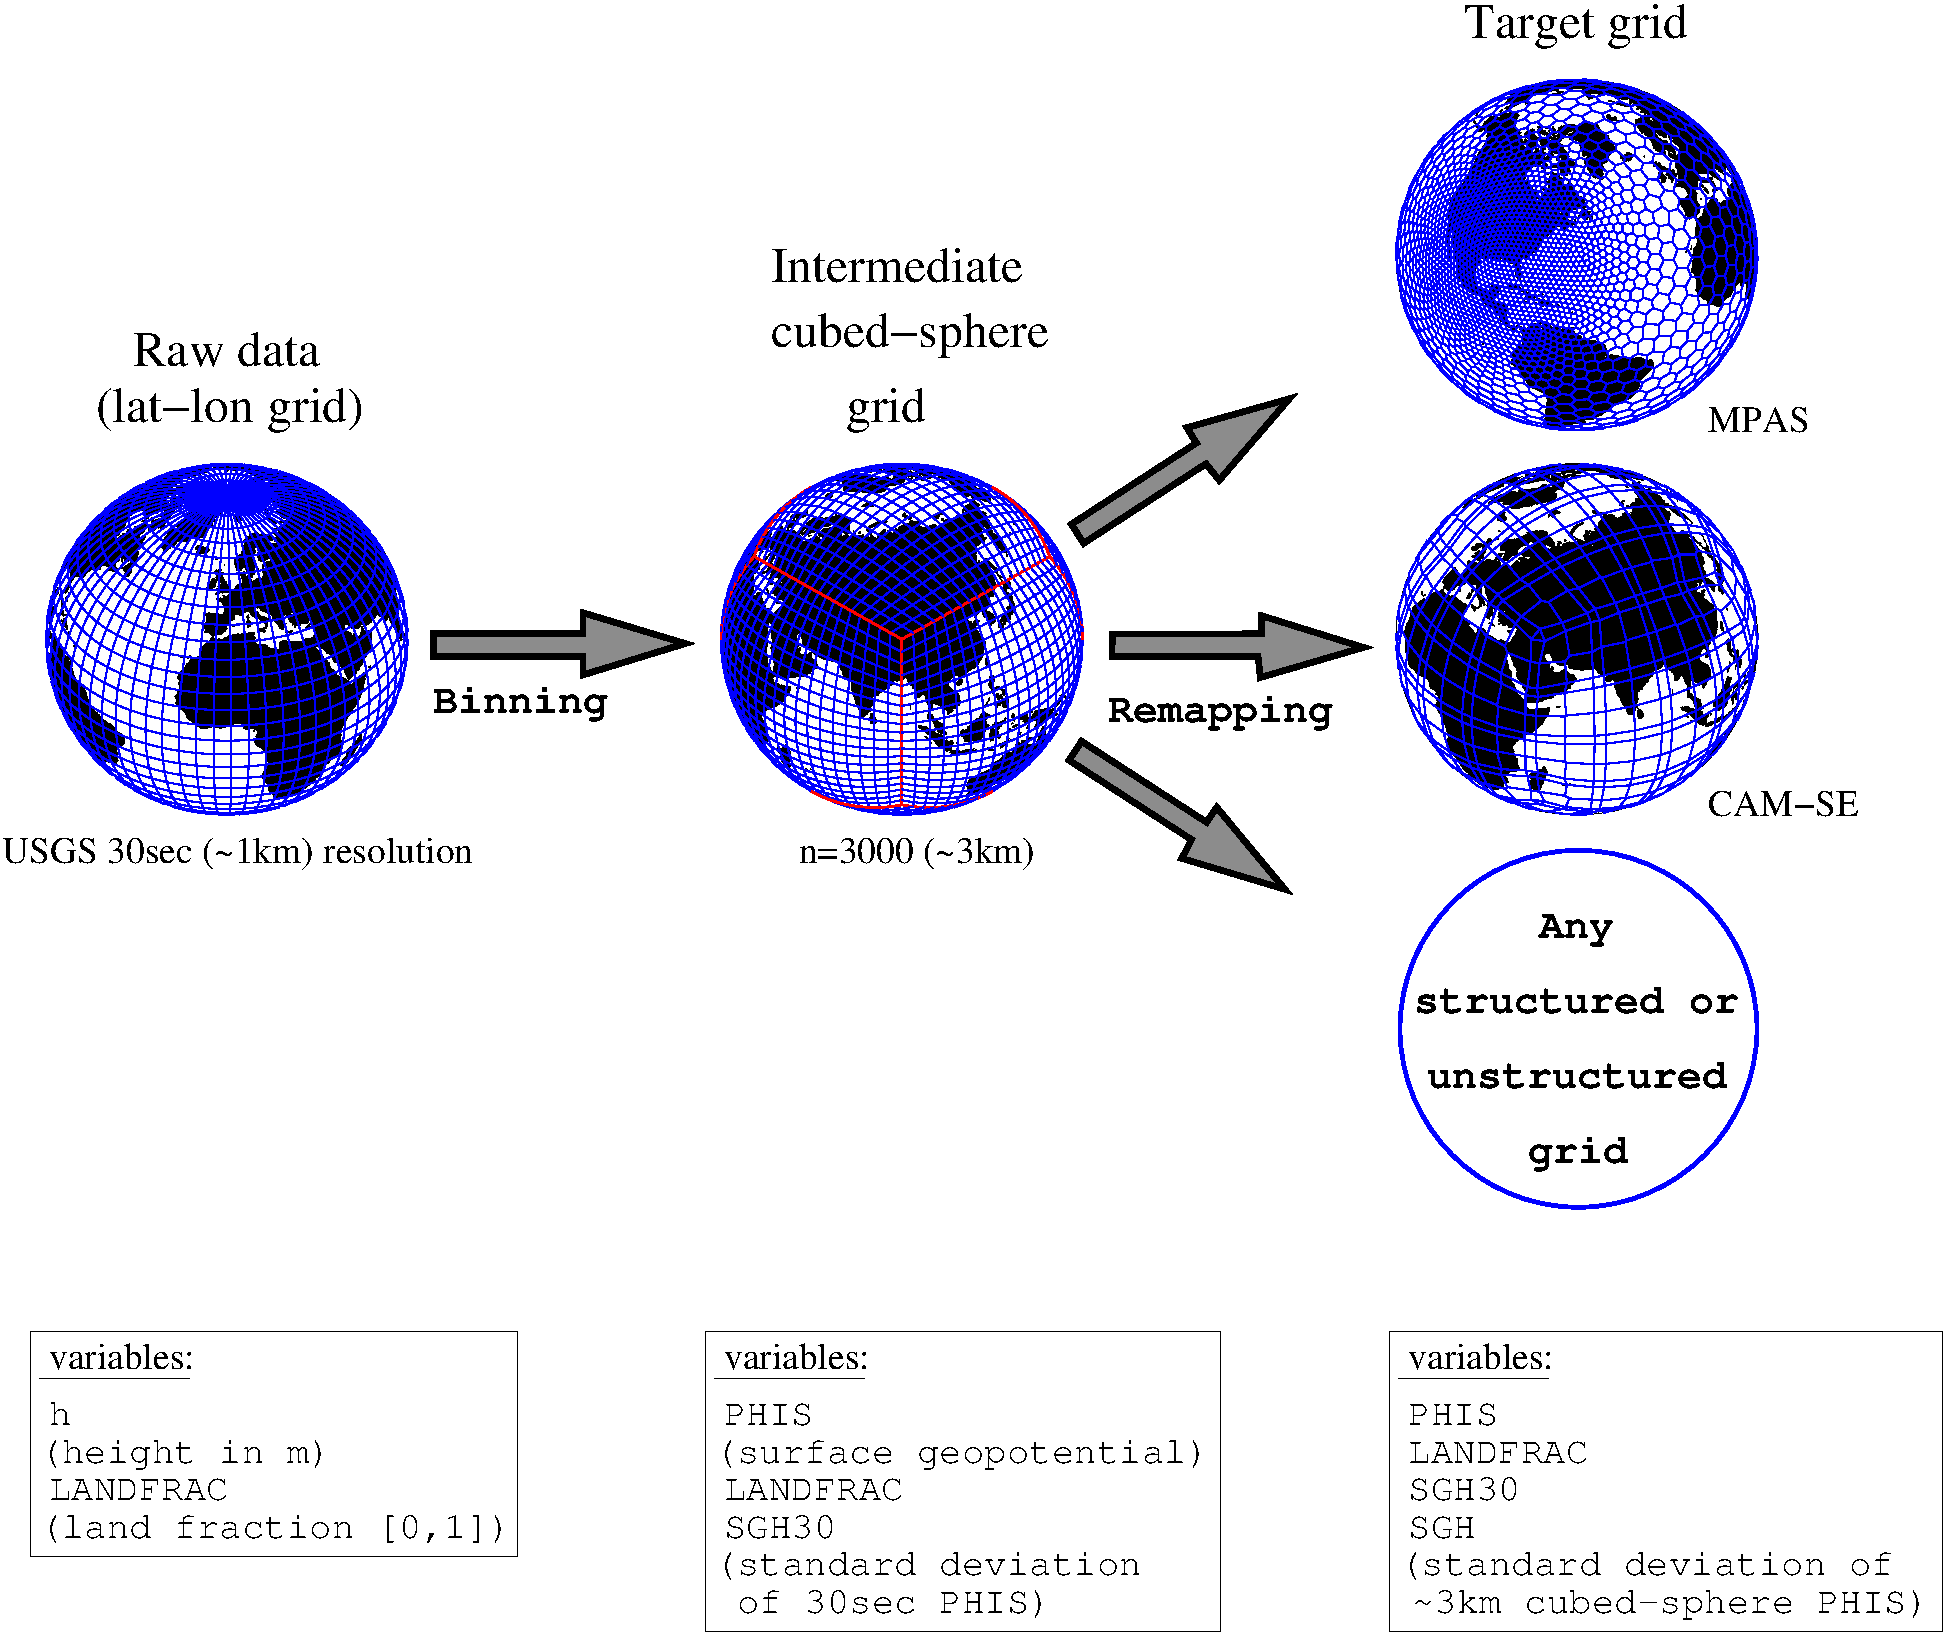
\includegraphics[width=12cm]{fig/schematic}
\end{center}
  \caption{A schematic showing the regridding procedure.}\label{fig:schematic}
\end{figure*}

Any quasi-uniform spherical grid could, in theory, be used for the separation of scales. For reasons that will become clear we have chosen to use a gnomonic cubed-sphere grid resulting from an  equi-angular gnomonic (central) projection
\begin{equation}
\label{eq:GnomonicCoordinates}
x=r \, \tan \alpha \quad \mbox{and} \quad y=r \, \tan \beta; \quad
    \alpha,\beta \in \left[ -\frac{\pi}{4},\frac{\pi}{4}\right],
\end{equation}
%
% next 6 lines are copied from JCP paper - rephrase
%
\citep{RIP1996JCP} where $\alpha$ and $\beta$ are central angles in each coordinate direction, $r=R/\sqrt{3}$ and $R$ is the radius of the Earth. A point on the sphere is identified with the three-element vector $(x,y,\nu)$, where $\nu$ is the panel index. Hence the physical domain $S$ (sphere) is represented by the gnomonic (central) projection of the cubed-sphere faces, $\Omega^{(\nu)}=[-1,1]^2$, $\nu = 1,2,\dots,6$, and the non-overlapping panel domains $\Omega^{(\nu)}$ span the entire sphere: $S=\bigcup_{\nu=1}^6\Omega^{(\nu)}$. The cube  edges, however, are discontinuous. Note that any straight line on the gnomonic projection $(x,y,\nu)$  corresponds to a great-circle arc on the sphere. In the discretized scheme we let the number of cells along a coordinate axis be $N_c$ so that the total number of cells in the global domain is $6\times N_c^2$. The grid lines are separated by the same angle $\Delta \alpha=\Delta \beta=\tfrac{\pi}{2\, N_c}$ in each coordinate direction.

For notational simplicity the cubed-sphere cells are identified with one index $i$ and the relationship between $i$ and $(icube,jcube,\nu)$ is given by 
\begin{equation}
i=icube+(jcube-1)\, N_c+(\nu-1)\, N_c^2,
\end{equation}
where $(icube,jcube)\in [1,..,N_c]^2$ and $\nu \in [1,2,..,6]$. In terms of central angles the cubed-sphere grid cell $i$ is defined as
\begin{multline}
A_i= [(icube-1)\Delta \alpha-\pi/4,icube\Delta \alpha-\pi/4]\times\\
 [(jcube-1)\Delta \beta-\pi/4,jcube\Delta \beta-\pi/4],
\end{multline}
and $\Delta A_i$ denotes the spherical area. A formula for the spherical area $\Delta A_i$ of a grid cell on the gnomonical cubed-sphere grid can be found in Appendix C of \citet{LN2008MWR} (note that equation C3 is missing $\\acos$ on the right-hand side). A quasi-uniform approximately 3km resolution is obtained by using $N_c=3000$. For more details on the construction of the gnomonic grid see, e.g., \cite{LNU2010JCP}.
%
%
%
\subsubsection{Step 1: raw elevation data to intermediate cubed-sphere grid ($\Lambda \rightarrow A$)}\label{sec:step1}
The `raw' elevation data is usually from a digital elevation model (DEM) such as the GTOPO30 30 arc second global dataset from the United States Geological Survey \citep[USGS][]{USGS} defined on an approximately 1km regular latitude-longitude grid. Several newer and higher resolution elevation datasets are available such as the NASA Shuttle Radar Topographic Mission (SRTM) DEM data \citep{SRTM}. The SRTM data, however, is only near-global (up to 60$^\circ$ North and South). In the remainder of this paper we assume that the raw elevation data is the USGS 30 arc second data.

The center of the regular latitude-longitude grid cells are denoted $(\lambda_{ilon},\theta_{jlat})$, $ilon=1,..., nlon$, $jlat=1, ..., nlat$. For the USGS dataset used here $nlon=43200$ and $nlat=21600$. As for the cubed-sphere we use one index $j$ to reference the grid cells
\begin{equation}
j=ilon+(jlat-1)\times nlon, \quad j\in [1, ..., N_r],
\end{equation} 
where $N_r=nlon\times nlat$. The spherical area of grid cell $\Lambda_j$ is denoted $\Delta \Lambda_j$ and the average elevation in cell $j$ is given by $\overline{h}^{(usgs)}_j$ 

This data is binned to the cubed-sphere intermediate grid by identifying in  which gnomonic cubed-sphere grid cell $(\lambda_{ilon},\theta_{jlat})$ is located. Due to the `Cartesian'-like structure of the cubed-sphere grid the search algorithm is straight forward:
\begin{itemize}
\item  use the transformation from latitude-longitude coordinates to central angle coordinates described in the Appendix of \cite{NTL2005MWRb} to compute the central angles $(\alpha, \beta)$ corresponding to the mid-point of the latitude-longitude grid cell $(\lambda_{ilon},\theta_{jlat})$.  [more details on algorithm z]
\item the indices of the cubed-sphere cell in which the center of the latitude-longitude grid cell is located is given by  
\begin{eqnarray*} 
icube &=& \verb+CEILING+\left(\frac{\alpha + \frac{\pi}{4}}{\Delta \alpha}\right),\\
jcube &=& \verb+CEILING+\left(\frac{\beta  + \frac{\pi}{4}}{\Delta \beta}\right),
\end{eqnarray*}
where the \verb+CEILING+($x$) function returns the smallest integer not less than $x$. 
\end{itemize}
The set of indices for which center points of regular latitude-longitude grid cells are located in gnomonic cubed-sphere cell $A_i$ is denoted ${\mathbb{S}}_i$. Note that since the USGS dataset is higher resolution that the cubed-sphere ${\mathbb{S}}_i$ is guaranteed to be non-empty. Through this binning process the approximate average elevation in cubed-sphere cell $i$ becomes
\begin{equation}
\overline{h}^{(cube)}_i=\frac{1}{\Delta A_i}\, \sum_{j\in {\mathbb{S}}_i}{\overline{h}}^{(usgs)}_j\Delta \Lambda_j.
\end{equation}
The binning process is straight forward since the cubed-sphere grid is essentially an equidistant Cartesian grid on each panel in terms of the central angle coordinates. This step could be replaced by rigorous remapping in terms of overlap areas between the regular latitude-longitude grid and the cubed-sphere grid using the geometrically exact algorithm of \citep{ULJ2009MWR} optimized for the regular latitude-longitude and gnomonic cubed-sphere grid pair or the more general remapping algorithm called SCRIP \citep{J1999MWR}.

The sub-grid-scale variance of elevation with respect to the cubed-sphere grid cell $i$ is
\begin{equation}
Var^{(tms)}_i=\frac{1}{\Delta A_i}\sum_{j\in {\mathbb{S}}_i} \left( \overline{h}_i^{(cube)}-{\overline{h}}^{(usgs)}_j\right)^2\, \Delta \Lambda_j.
\end{equation}

\begin{itemize}
\item mention the changes to raw data: Caspian sea, Antartica (why are these changes made?)
\end{itemize}

%
% show details of that algorithm form the code
%
%        call CubedSphereABPFromRLL(lon(i), lat(j), alpha, beta, ipanel)            
%       icube = CEILING((alpha + piq) / da)
%       jcube = CEILING((beta  + piq) / da)
%\begin{figure}[t]
%\center\includegraphics[width=35pc,angle=0]{fig/effect-of-binning}\\
%  \caption{Effect of binning (figure Curtesy of S.J. Lin (GFDL) [will be replaced with Figure from CAM data].)}\label{fig:nonconvex}
%\end{figure}
TODO: show a Figure illustrating the amount of smoothing performed by the binning!
%
\subsubsection{Step 2: cubed-sphere grid to target grid ($A\rightarrow \Omega$)}\label{sec:step2}
The cell averaged values of elevation and sub-grid-scale variances ($Var^{(tms)}$ and $Var^{(gwd)}$) on the target grid are computed by rigorously remapping the variables from the cubed-sphere grid to the target grid.  The remapping is performed using CSLAM (Conservative Semi-LAgrangian Multi-tracer transport scheme) technology \citep{LNU2010JCP} that has the option for performing higher-order remapping. It s possible to use large parts of the CSLAM technology since the source grid is a gnomonic cubed-sphere grid hence instead of remapping between the gnomonic cubed-sphere grid and a deformed Lagrangian grid, as done in CSLAM transport, the remapping is from the gnomonic cubed-sphere grid to any target grid constructed from great-circle arcs (the target grid `plays the role' of the Lagrangian grid). However, a couple of modifications where made to the CSLAM search algorithm. First of all, the target grid cells can have an arbitrary number of vertices whereas the CSLAM transport search algorithm assumes that the target grid consists of quadrilaterals and the number of overlap areas are determined by the deformation of the transporting velocity field. In the case of the remapping needed in this application the target grid consists of polygons with any number of vertices and the search is not constrained by the physical relation between regular and deformed upstream quadrilaterals. Secondly, the CSLAM search algorithm for transport assumes that the target grid cells are convex which is not necessarily the case for topography target grids. The CSLAM search algorithm has been modified to support non-convex cells that are, for example, encountered in variables resolution CAM-SE; essentially that means that any target grid cell may cross a gnonomic isoline (source grid line) more than twice as is the case for transport.
%\begin{figure}[t]
%\center\includegraphics[width=15pc,angle=0]{fig/non-convex-cell/1.pdf}\\
%  \caption{Non-convex cell from variable resolution CAM-SE.}\label{fig:nonconvex}
%\end{figure}

Let the target grid consist of $N_t$ grid cells $\Omega_k$, $k=1, ..., N_t$ with associated spherical area $\Delta \Omega_k$. The search algorithm for CSLAM is used to identify overlap areas between the target grid cell $\Omega_k$ and the cubed-sphere grid cells $A_\ell$, $\ell=1,..,N_c$. Denote the overlap area between $\Omega_k$ and $A_\ell$
\begin{equation}
\Omega_{k\ell}=\Omega_k \cap A_\ell,
\end{equation}
and let $\mathbb{L}_k$ denote the set of indices for which $\Omega_k \cap A_\ell$, $\ell=1,..,N_c$, is non-empty. Then the average elevation and variance used for TMS in target grid cell $k$ are given by
\begin{eqnarray}
\overline{h}^{(targ)}_k&=&\frac{1}{\Delta \Omega_k}\sum_{\ell\in {\mathbb{L}}_k}\overline{h}^{(cube)}_\ell\, \Delta \Omega_{k\ell},\\
\overline{Var}^{(tms)}_k&=&\frac{1}{\Delta \Omega_k}\sum_{\ell\in {\mathbb{L}}_k}\overline{Var}^{(tms)}_\ell\, \Delta \Omega_{k\ell},
\end{eqnarray}
respectively. The variance of the cubed-sphere data $\overline{h}^{(cube)}$ with respect to the target grid cell average values $\overline{h}^{(targ)}$ is given by
\begin{equation}
\overline{Var}^{(sgh)}_k=\frac{1}{\Delta \Omega_k}\sum_{\ell\in {\mathbb{L}}_k}\left( \overline{h}^{(targ)}_k-\overline{h}^{(cube)}_\ell\right)^2\, \Delta \Omega_{k\ell},
\end{equation}

\subsubsection{Smoothing of $\Phi_s$}\label{sec:smoothing}
Modeling groups, with the exception of the UK Met Office \citep{WBCJ2003QJRMS}, rarely publish their smoothing procedures and criteria for choosing one level of smoothing over another. It is likely that qualitative methods are used such as the elimination of visible noise in, e.g. vertical velocity, near topography rather than quantitative diagnostics. The amount of smoothing necessary to remove spurious noise in, e.g. vertical velocity, depends on the amount of inherent or explicit numerical diffusion in the dynamical core \citep[e.g., ][]{L2011IJHPC}. In the NCAR-DOE CESM (Community Earth System Model) CAM-FV \citep[Community Atmosphere Model - Finite-Volume; ][]{L2004MWR} the highest wave-numbers are removed by mapping $\Phi_s$ (surface geopotential) to a regular latitude-longitude grid that is half the resolution of the desired model resolution, and then mapped back to the model grid by one-dimensional remaps along latitudes and longitudes, respectively, using the PPM (Piecewise Parabolic Method) with monotone filtering. In CAM-SE \citep[Community Atmosphere Model - Spectral-Elements;][]{DetAl2012IJHPCA,CAM5} the surface geopotential is smoothed by multiple applications of the CAM-SE Laplace operator combined with a bounds preserving limiter. Figure \ref{fig:topo-smoothing-height} shows different levels of smoothing of surface height for CAM-SE and for comparison CAM-FV. It can clearly be seen that there are large differences between the height of the mountains used in the dynamical core. 


Up to model developer ...\\

Describe internal smoothing algorithm ,,,,

\subsubsection{Algorithm for determining the dominant orientation of sub-grid topography}\label{sec:sub-orient}
Our algorithm for determining the dominant orientation of sub-grid topography is relatively straightforward.  We begin with 3 km topography on the intermediate cubed-sphere grid and compute an extension of each panel on the cubed-sphere via high-order interpolation so that each panel can numerically be treated essentially as a Cartesian computational domain. An outer/model scale ($L$) is selected.  A high-pass filter is optionally applied to remove larger scales.  We then take a square of topography $h(x,y)$ with dimension $L$ and rotate it through 16 test angles $\xi_i$.  `Padding' is used to avoid corner effects.  In each test rotation a `Y' average is taken to generate a ridge profile $h_i(x)$ at angle $\xi_i$.  The ratio of the variance of $h_i$ to the total 2D variance in $h(x,y)$ is computed.  The angle for which this ratio is greatest is designated as the dominant topographic orientation for the sub-grid topography in the $LxL$ domain of $h(x,y)$.  This is done at regular intervals separated by $L$ over the entire globe.  The angle and other topographic parameters can then be mapped from the cubed sphere grid with resolution $L$ to arbitrary model grids using the new topography software already available in CAM.  Preliminary results from our algorithm are presented in Figure \ref{fig:dsgso}.
\begin{figure}[tb]
\center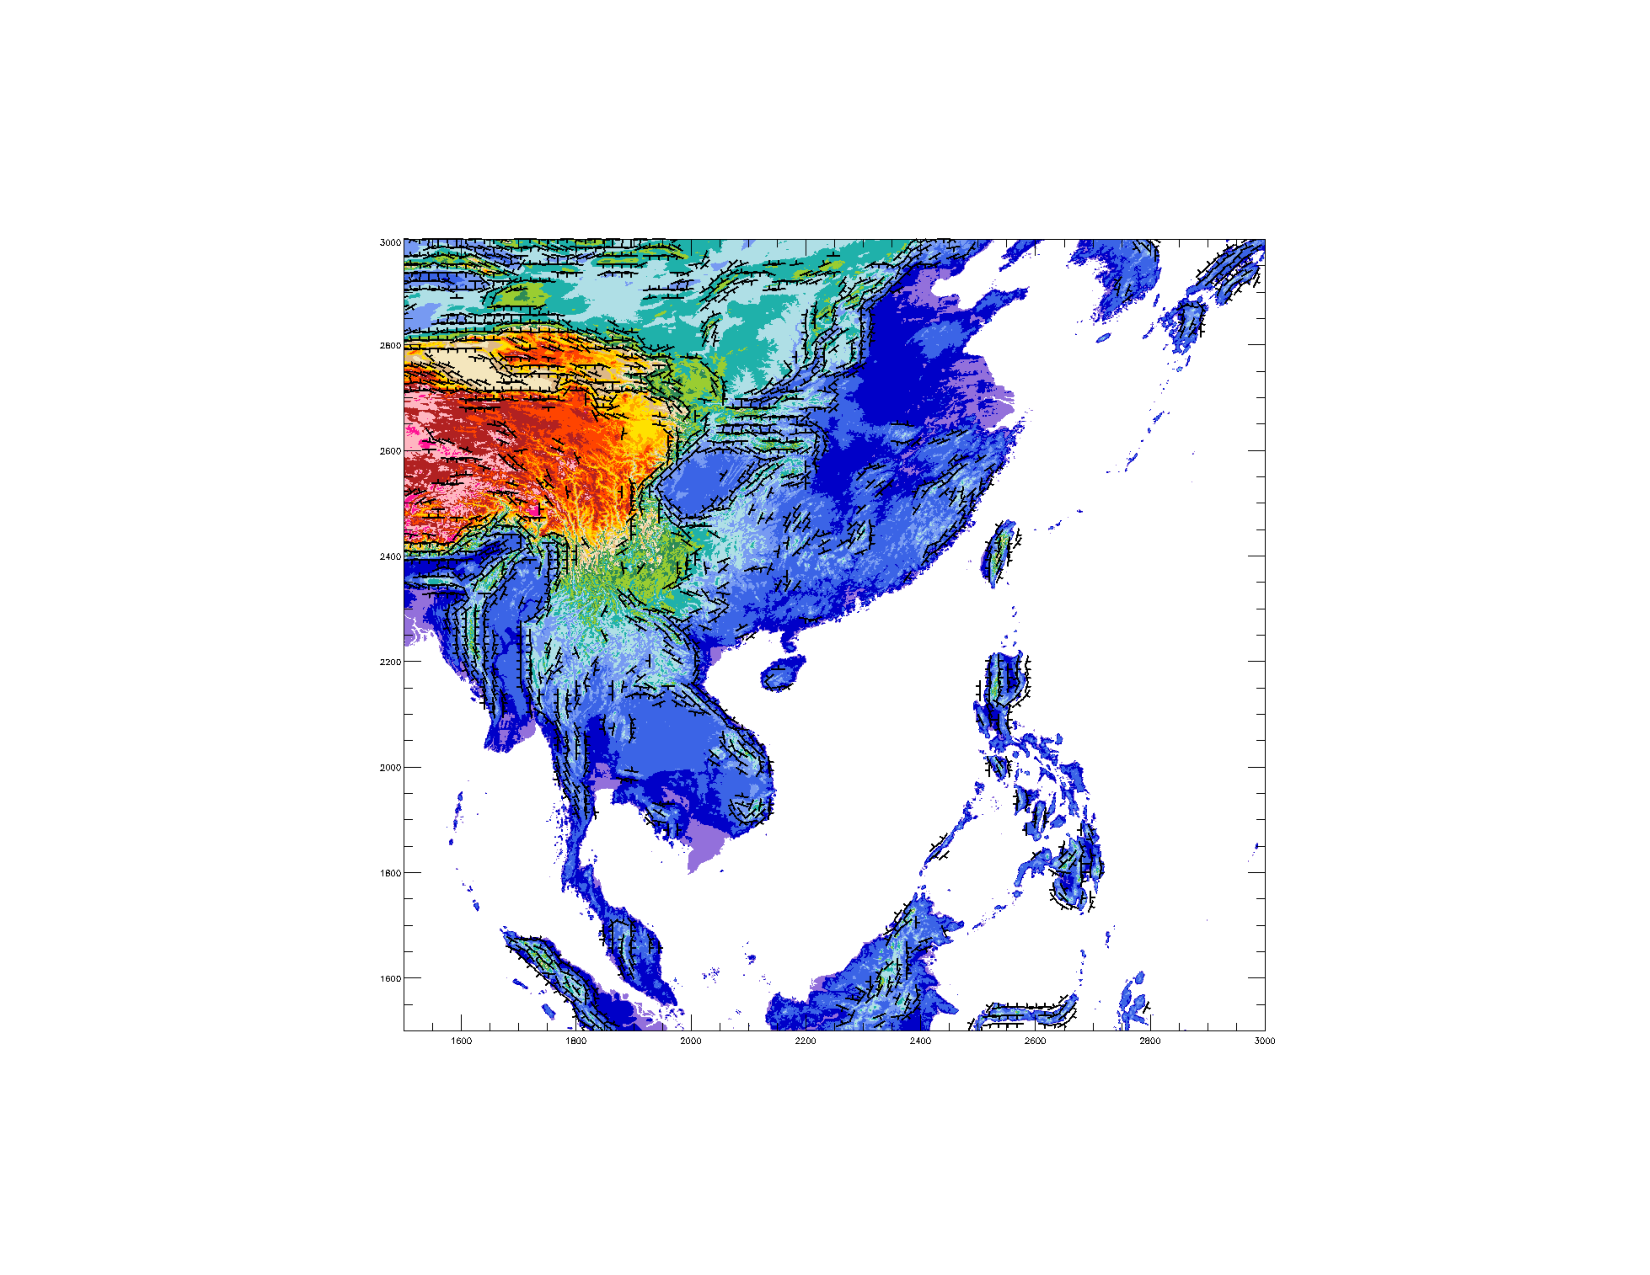
\includegraphics[width=20pc,angle=0]{fig/dominant-sub-grid-oro.pdf}
  \caption{Topography of southeast Asia (color) and diagnosed ridges (black symbols). An outer scale of 50 km is used. Only ridges explaining 50\% or more of total 2D variance and possessing maximum vertical displacement of more than 500 m are shown.  Long axes of symbols show ridge crests, short appendages indicate direction of greater descent.}\label{fig:dsgso}
\end{figure} 

\section{Results}
\begin{figure*}[t]
\vspace*{2mm}
\begin{center}
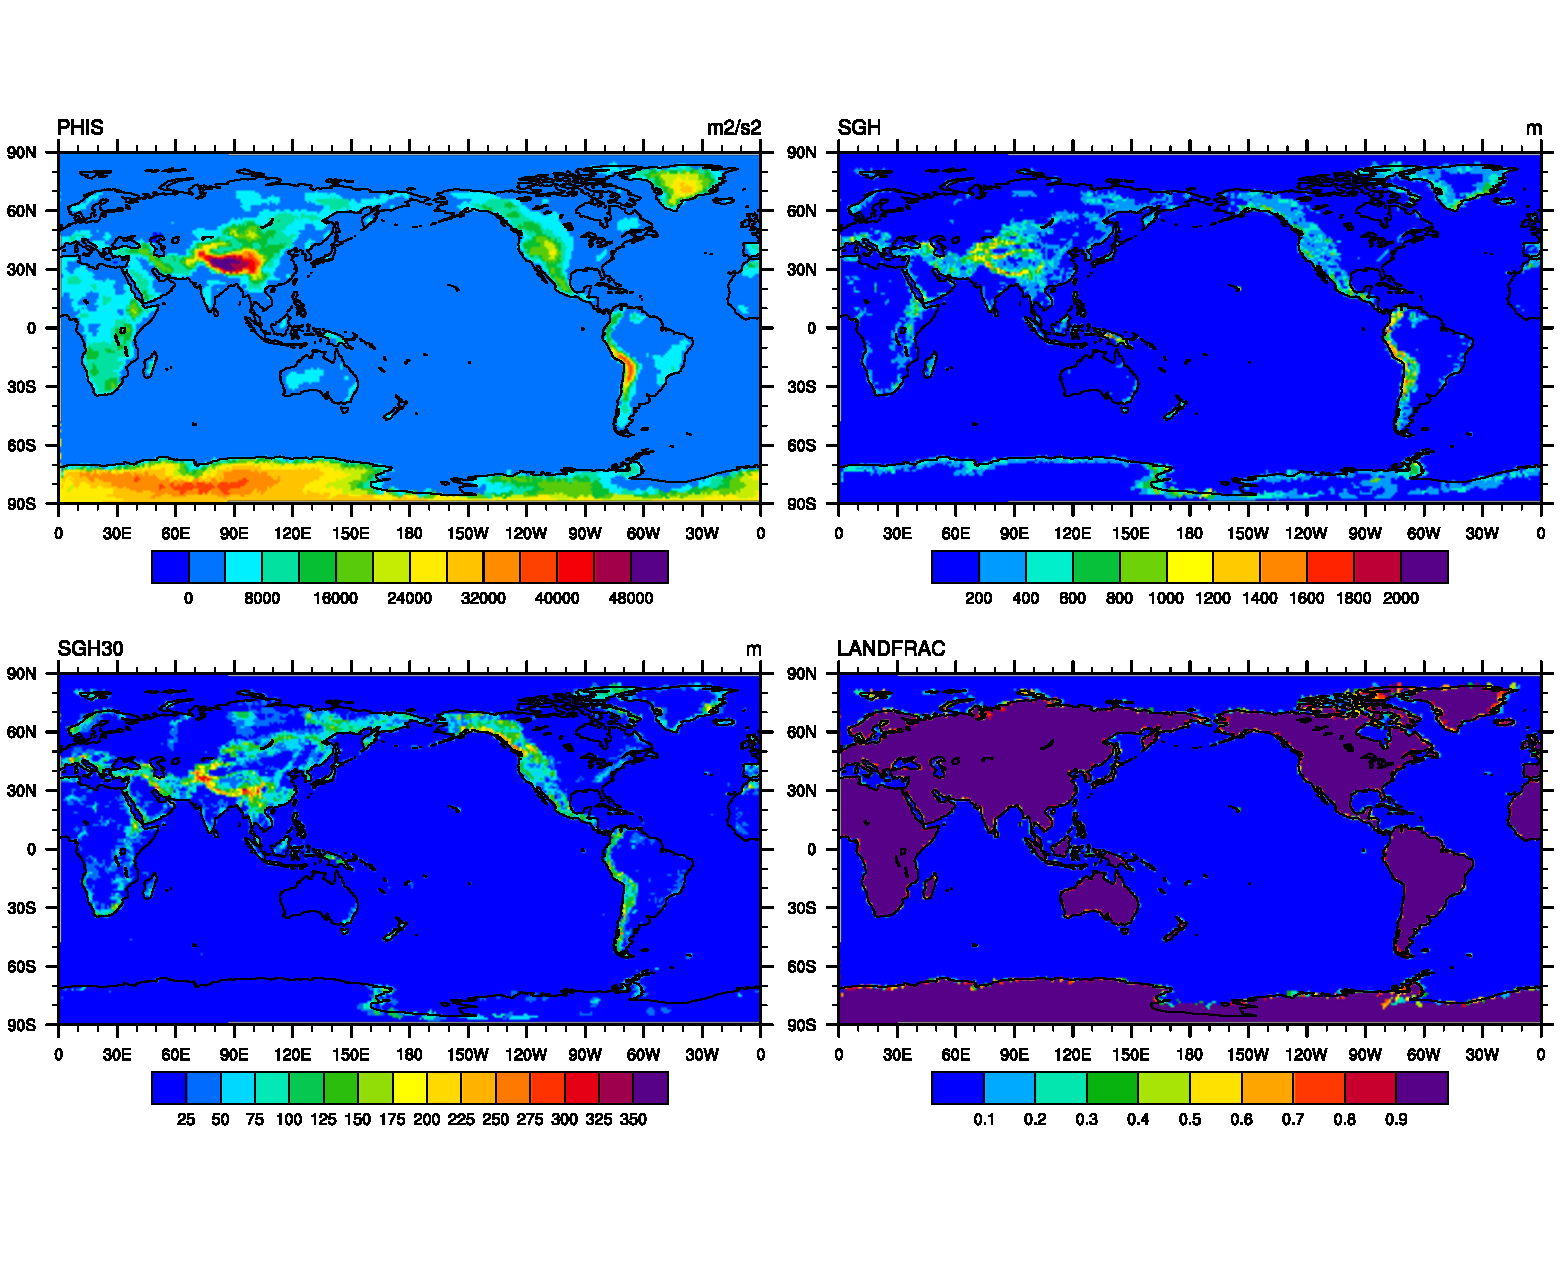
\includegraphics[width=12cm]{fig/topo-vars_global}
\end{center}
  \caption{Surface geopotential $\Phi_s$ (upper left), $SGH$ (upper right), $SGH30$ (lower left) and $LANDFRAC$ (lower right) for CAM-SE NE30NP4 resolution. The data is plotted on the native grid.}\label{fig:topo-vars}
\end{figure*}


TEXT

\subsection{Sample topography smoothing experiments with CAM-SE}
HOMME \citep[High-Order Method Modeling Environment; ][]{HOMME,DetAl2005IJHPCA}\\




\begin{figure}[t]
\vspace*{2mm}
\begin{center}
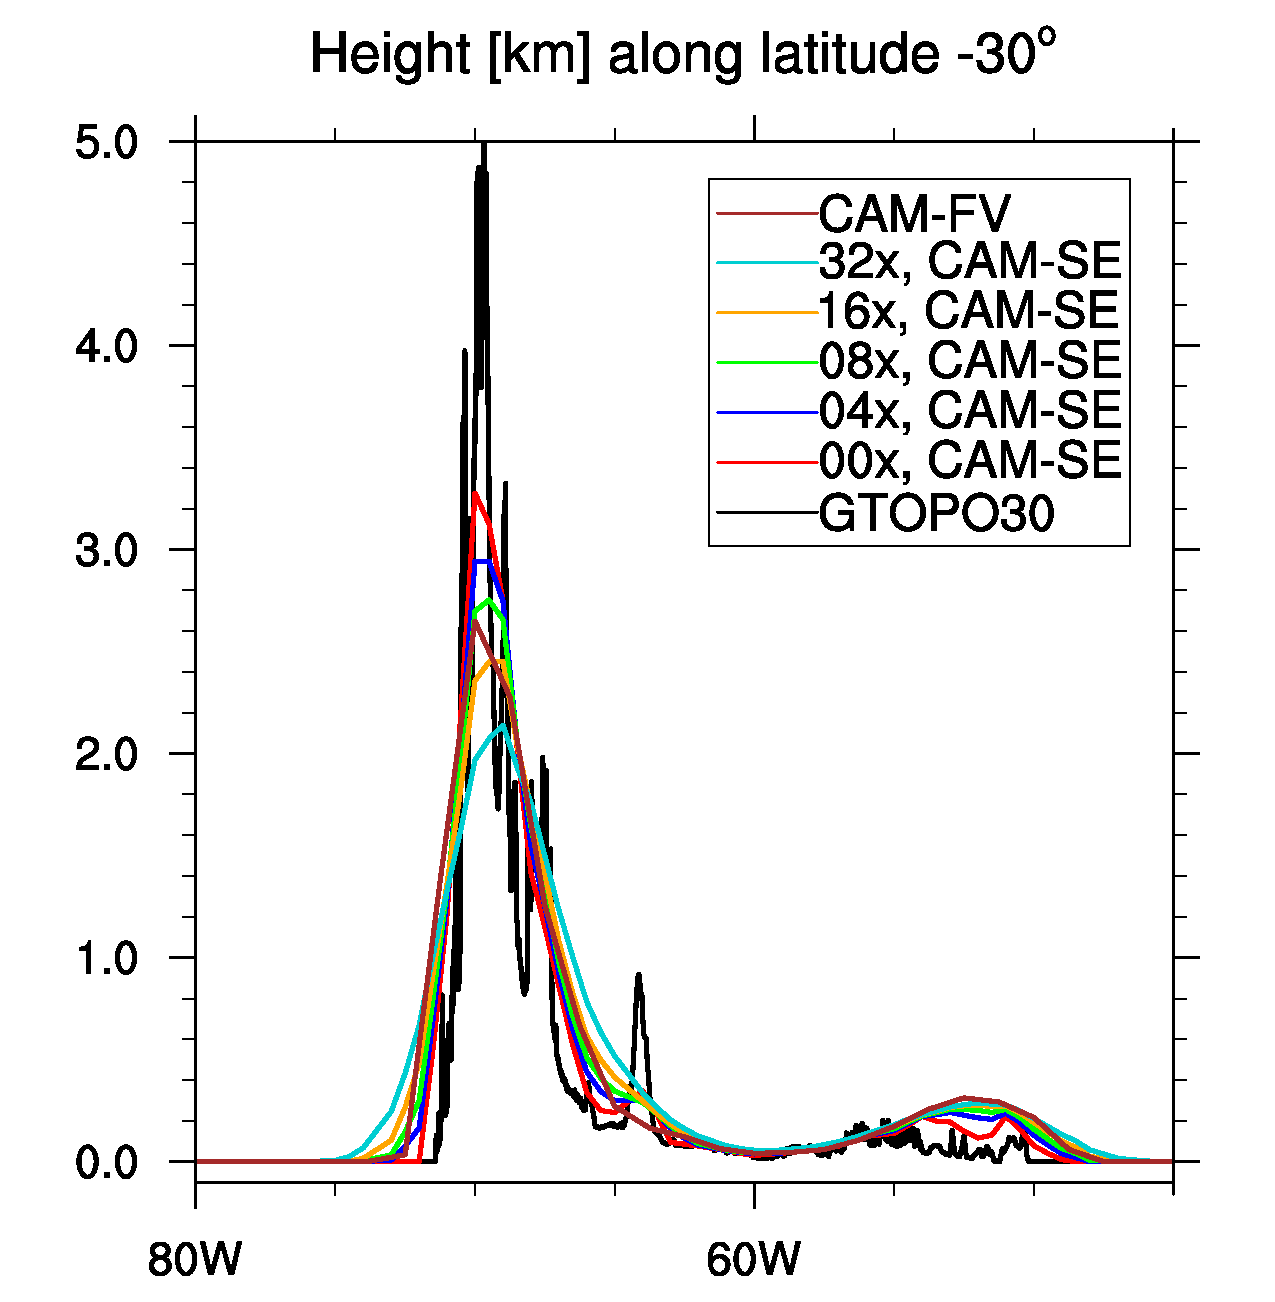
\includegraphics[width=8.3cm]{fig/topo-smoothing-height}
\end{center}
  \caption{Surface elevation in kilometers for a cross section along latitude $30^\circ$S (through Andes mountain range) for different representations of surface elevation. Labels `4x', `8x', '16x' and `32x', refer to different levels of smoothing, more precisely, four, eight, sixteen and thirtytwo applications of a `Laplacian' smoothing operator in CAM-SE, respectively. Label `FV $0.9^\circ \times 1.25^\circ$' refers to the topography used in CAM-FV. `0x' is the unsmoothed topography on an approximately $1^\circ$ grid.}\label{fig:topo-smoothing-height}
\end{figure}
\begin{figure*}[t]
\vspace*{2mm}
\begin{center}
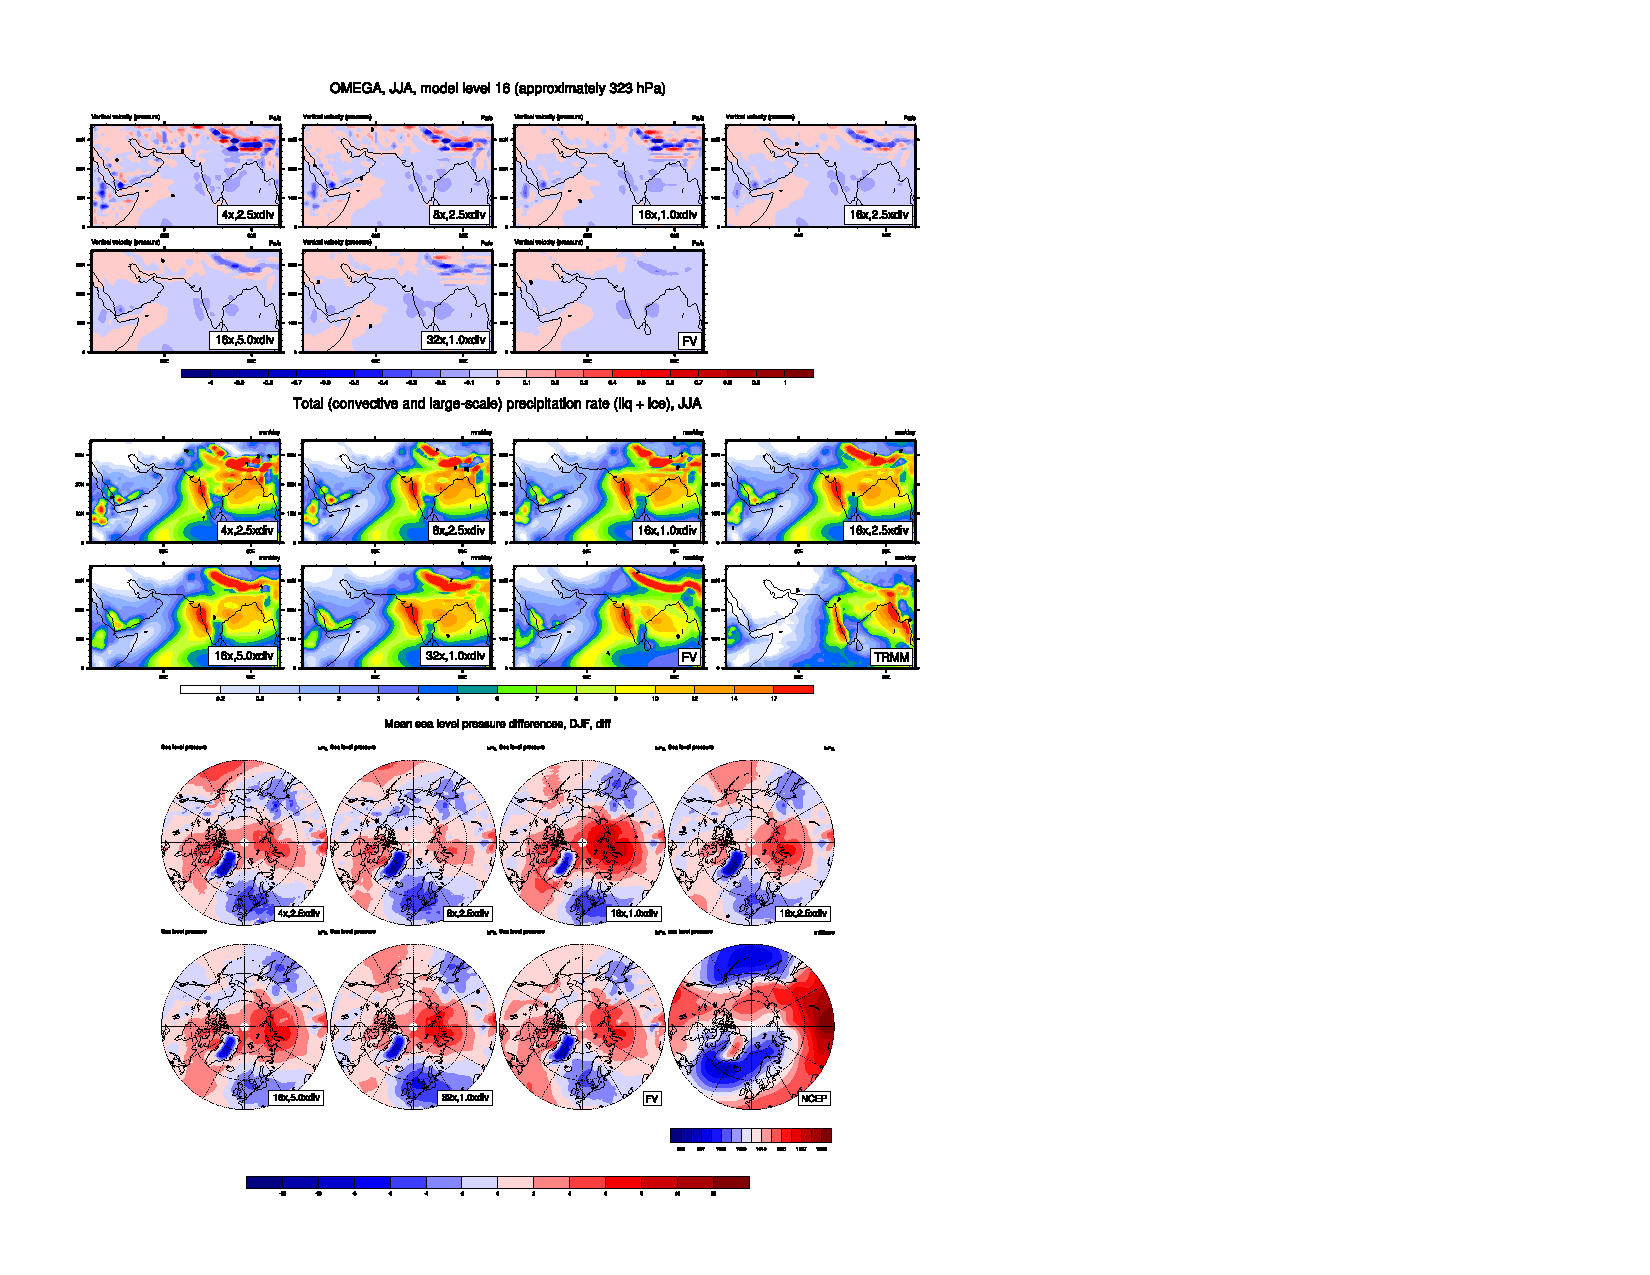
\includegraphics[width=12cm]{fig/topo-smoothing-experiments.pdf}
\end{center}
  \caption{Diagnostics for 30 year AMIP simulations with CAM5.2. Upper, middle and lower group of plots are  model level 16 vertical velocity, total precipitation rate and mean sea level pressure differences, respectively, Except for the two right-most plots on the second row of each group of plots, the diagnostics are for CAM-SE with different amounts of smoothing of $\Phi_s$ and different levels of divergence damping. The amount of smoothing follows the same notation as Fig. \ref{fig:topo-smoothing-height} (right) and $1.0 x div$, $2.5 x div$, $5.0 x div$ refers to increasing divergence damping by a factor 1,0, 2.5, and 5.0, respectively. The second right-most plot on each group of plots (labeled FV) show results for CAM-FV. Lower right plot in the second and third group of plots show TRMM observations and NCEP reanalysis data, respectively.}\label{fig:topo-smoothing-exp}
\end{figure*}

\begin{figure*}[t]
\vspace*{2mm}
\begin{center}
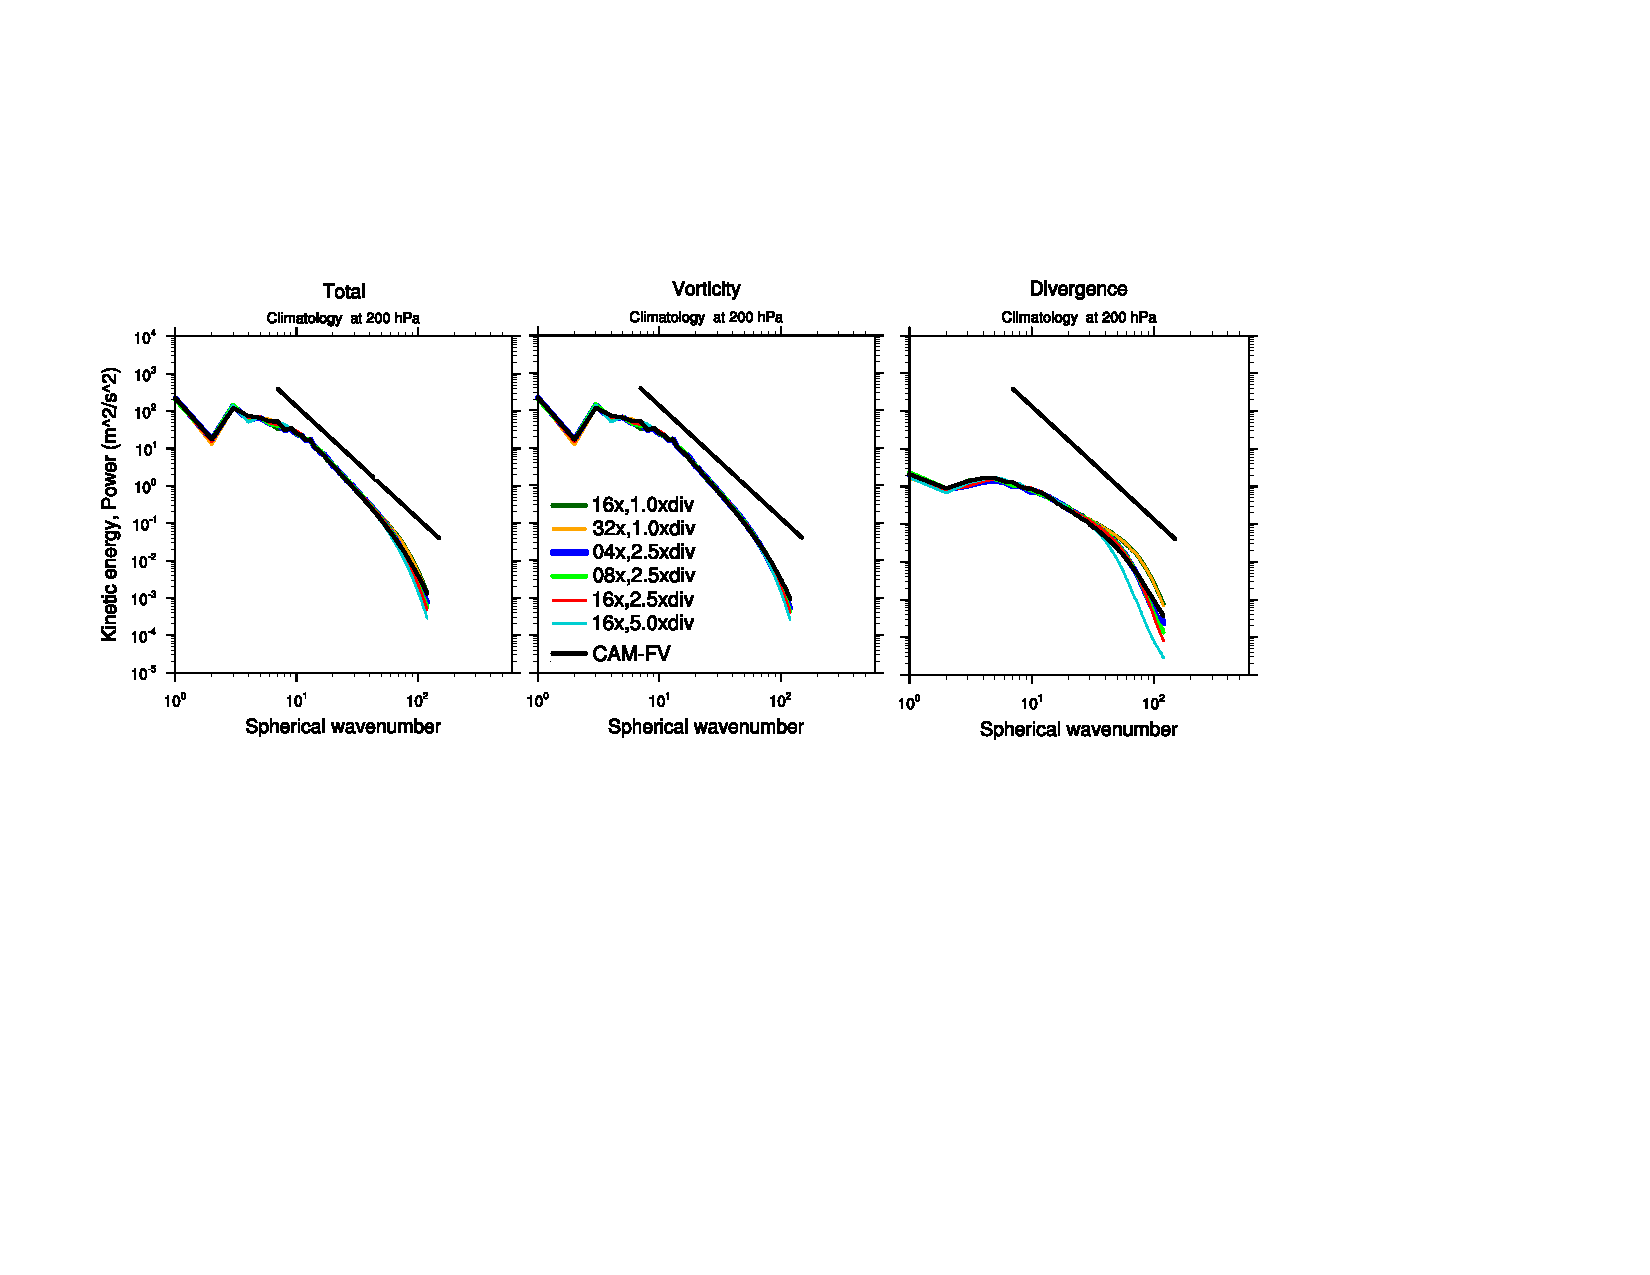
\includegraphics[width=12cm]{fig/TKE-fig}
\end{center}
  \caption{(left) Total kinetic energy spectrum for the velocity field at 200hPa as a function of spherical wavenumber $k$ for CAM-FV and different configurations of CAM-SE. The labeling for the CAM-SE configurations is the same as in Figure \ref{fig:topo-smoothing-exp}. The solid-straight black line indicates the $k^{-3}$ reference slope \citep{NG1985JAS}. The middle and right plots show the kinetic energy partitioned into divergent and rotational modes, respectively. The spectra have been computed using daily instantaneous wind and surface pressure data for a 2 month period.}\label{fig:tke}
\end{figure*}




Figure \ref{fig:topo-smoothing-exp} shows results from AMIP simulations with CAM-SE using different levels of $\Phi_s$ smoothing and numerical diffusion of divergent modes. Spurious noise near steep topography is very apparent for certain model configurations and affects important hydrological fields such as precipitation; even surface pressure varies significantly among the model configurations (not shown) which, in turn, affects sea ice extent and other important climate variables. 

While it is necessary to smooth topography to remove spurious grid-scale noise, it introduces two problems. Filtering will typically raise ocean points near step topography to non-zero elevation. Perhaps the most striking example is the Andes mountain range that extends one or two grid cells into the Pacific after the filtering operation (see, e.g., Figure \ref{fig:oro-spectra} right). Ocean and land points are treated separately in weather/climate models so raised sea-points may potentially be problematic. Secondly, the filtering will generally reduce the height of local topographic maxima and given the importance of barrier heights in atmospheric dynamics, this could be a problem for the global angular momentum budget and could fundamentally change the flow. 

To capture the barrier effect (blocking) that is sub-grid scale with respect to the smoothed topography, one may use {\em{envelope topography}} that adjusts the surface height with sub-grid scale topographic variance \citep{WTS1983QJRMS}. Loosely speaking, the peak heights are raised. A similar approach, but implemented as variational filtering, is taken in \cite{RTS2006QJRMS}; this method also imposes additional constraints such as enforcing zero elevation over ocean masks.

 
As mentioned above it is not straight forward to determine how to smooth topography. One approach is to try different filtering methods in the full model and evaluate the results in weather forecasts or longer climate simulations \citep{NSM1994JC,B1995QJRMS,H1996JC}. While this approach is certainly valuable, clearly the size of the Gibbs oscillations in global spectral models is reduced by smoothing topography, it does not take into account the interaction between the resolved-scale flow (dynamical core) and parameterizations of sub-grid scale processes (e.g., gravity wave drag, turbulent mountain stress). This interaction can be difficult to predict and commonly the sub-grid scale parameterization have been tuned over a number of years with the `default' smoothed surface elevation. Hence, this methodology runs the risk of deeming one smoothing less accurate than another due to lack of optimum tuning (and/or complexity) of the parameterizations.

Another approach is to use idealized simulation with no parameterizations to determine what scales are adequately resolved and which are poorly resolved. \cite{DB2001QJRMS} kept the physical scale of an idealized two-dimensional and three-dimensional isolated hill fixed and observed how the coarser resolution results differ from the high-resolution simulation. This can then provide guide-lines on how to smooth topography in the full model. Similar idealized (shallow water) experiments where used in \cite{RTS2006QJRMS} to optimally smooth topography. While these idealized tests provide a `cleaner' approach to smoothing terrain, they do not consider the coupling with sub-grid scale processes.







TEXT

\subsubsection{HEADING}
TEXT




\conclusions  %% \conclusions[modified heading if necessary]
TEXT




\appendix
\section{\\ \\ \hspace*{-7mm} Grid descriptor NetCDF file}    %% Appendix A

\subsection{asdf}                               %% Appendix A1, A2, etc.




\begin{acknowledgements}
NCAR is sponsored by the National Science Foundation (NSF). Thanks to DOE ...
\end{acknowledgements}



\bibliographystyle{copernicus}
\bibliography{bib}

%\begin{thebibliography}{}
%
%\bibitem[AUTHOR(YEAR)]{LABEL}
%REFERENCE 1
%
%\bibitem[AUTHOR(YEAR)]{LABEL}
%REFERENCE 2
%
%...
%
%\end{thebibliography}


%% Literature citations
%% command                        & example result
%% \citet{jones90}|               & Jones et al.\ (1990)
%% \citep{jones90}|               & (Jones et al., 1990)
%% \citep{jones90,jones93}|       & (Jones et al., 1990, 1993)
%% \citep[p.~32]{jones90}|        & (Jones et al., 1990, p.~32)
%% \citep[e.g.,][]{jones90}|      & (e.g., Jones et al., 1990)
%% \citep[e.g.,][p.~32]{jones90}| & (e.g., Jones et al., 1990, p.~32)
%% \citeauthor{jones90}|          & Jones et al.
%% \citeyear{jones90}|            & 1990






%% FIGURES %%%%%%%%%%%%%%%%%%%%%%%%%%%%%%%%%%%%%%%%%%%%%%%%%%%%%%%%%%%%%%%%%%%%


%% ONE-COLUMN FIGURES

%f
%\begin{figure}[t]
%\vspace*{2mm}
%\begin{center}
%\includegraphics[width=8.3cm]{FILE NAME}
%\end{center}
%\caption{TEXT}
%\end{figure}



%% TWO-COLUMN FIGURES

%f
%\begin{figure*}[t]
%\vspace*{2mm}
%\begin{center}
%\includegraphics[width=12cm]{FILE NAME}
%\end{center}
%\caption{TEXT}
%\end{figure*}


%% TABLES %%%%%%%%%%%%%%%%%%%%%%%%%%%%%%%%%%%%%%%%%%%%%%%%%%%%%%%%%%%%%%%%%%%%


%% ONE-COLUMN TABLE

%t
%\begin{table}[t]
%\caption{TEXT}
%\vskip4mm
%\centering
%\begin{tabular}{column = lcr}
%\tophline
%
%\middlehline
%
%\bottomhline
%\end{tabular}
%\end{table}


%% TWO-COLUMN TABLE

%t
%\begin{table*}[t]
%\caption{TEXT}
%\vskip4mm
%\centering
%\begin{tabular}{column = lcr}
%\tophline
%
%\middlehline
%
%\bottomhline
%\end{tabular}
%\end{table*}


%% The different columns must be seperated with a & command and should
%% end with \\ to identify the column brake.

%%%%%%%%%%%%%%%%%%%%%%%%%%%%%%%%%%%%%%%%%%%%%%%%%%%%%%%%%%%%%%%%%%%%%%%%%%%%%%


%% If figures and tables must be numbered 1a, 1b, etc. the following command
%% should be inserted before the begin{} command.

%\addtocounter{figure}{-1}\renewcommand{\thefigure}{\arabic{figure}a}


\end{document}
